\documentclass[../../main.tex]{subfiles}

\graphicspath{{\subfix{images/}}}

\begin{document}

\addtocontents{toc}{\protect\newpage}
\chapter{Proiectarea, Implementarea și \\Testarea Platformei}
\label{ch:platform}

Plecând de la informațiile expuse în capitolul anterior, de la cele referitoare la arhitecturile de procesoare și ajungând până la cele despre învățarea automată cu ajutorul unor algoritmi dedicați, am putut deduce cerințele software și arhitectura unui sistem în care inteligența artificială este folosită pentru a îmbunătăți procesul de analiză automată a programelor malițioase.

\section{Cerințe Software}
\label{sec:platform_requirements}

Pentru definirea \textbf{cerințelor software}, ne-am limitat la un context al organiza\-țiilor mici și mijlocii, care doresc fie un strat suplimentar de securitate în infra\-structura proprie, fie trierea unui flux de fișiere posibil malițioase, trimise spre a fi analizate manual. Această abordare favorizează deducerea nevoilor esențiale pentru o platformă de acest tip, putând ulterior finalizării acestei lucrări să studiem cum ele se pot scala unui cadru mai larg, pentru organizațiile de dimensiuni mari.

\subsection{Cerințe Funcționale}

Din punct de vedere al \textbf{cerințelor funcționale}, platforma trebuie să fie ușor de gestionat de către un \textbf{administrator de infrastructură organizațională}, fără ca acesta să aibă nevoie de cunoștințe specifice, în domeniile de analiză de programe malițioase și de ingineria datelor. Sunt permise acțiuni de \textbf{instalare a platformei} pe un server, de \textbf{dezinstalare} și de \textbf{actualizare}, cu păstrarea compatibilității cu versiunea anterioară (pentru comenzile interfeței de administrator și pentru API) și cu datele existente (configurație, seturi de date construite și modele antrenate).

Funcționalitățile pe care platforma trebuie să le asigure pot fi deduse din suita de utilizatori pe care o poate avea. În primul rând, o persoană având cunoștințele specifice, menționate anterior, va ocupa o poziție de \textbf{administrator al platformei}. Ea va folosi arhitectura de servere pentru a \textbf{lucra cu exemplarele benigne și malițioase} și pentru a \textbf{gestiona seturi de date și modele}. Pe de altă parte, clienții sunt reprezentați de:

\begin{itemize}
    \item \textbfit{Simpli membrii ai organizației}: Ei \textbf{scanează fișiere} aflate în posesia lor (de exemplu, un fișier Word descărcat de pe Internet, pe stația de lucru) prin intermediul unui produs software accesibil lor.
    \item \textbfit{Membrii ai departamentelor de securitatea informației} (inclusiv analiști de programe malițioase): Ei își formează o premisă pe baza rezultatului returnat de modelele antrenate. Acest lucru ajută la \textbf{luarea unei decizii rapide} în privința unui fișier intrat în rețeaua organizațională (de exemplu, de blocare la nivel de \textit{firewall}) și la \textbf{stabilirea unei ipoteze} premergătoare unei analize manuale, amănunțite.
    \item \textbfit{Alte sisteme ale organizației}: Folosesc API-ul pentru \textbf{scanarea a\-utomată a fișierelor}. Un exemplu aici ar fi integrarea cu un server de \textit{email}, pentru scanarea atașamentelor tuturor \textit{email}-urilor primite de către angajați.
\end{itemize}

\subsection{Cerințe Nefuncționale}

Trecând la \textbf{criteriile} pe care le-am avut în considerare \textbf{în dezvoltarea și evaluarea platformei}, acestea sunt după cum urmează:

\begin{itemize}
    \item \textbfit{Performanțe bune ale modelelor antrenate}: Modelele antrenate în cadrul platformei sunt calitative, conform unor metrici de evaluare specifice învățării automate, mai exact specifice regresiei și clasificării.
    \item \textbfit{Programare în Python}: Limbajul de programare folosit pentru implementarea platformei este Python. Motivul este reprezentat de avantajele pe care acesta le prezintă, dintre care putem aminti disponibilitatea pe o varietate de platforme (engl. "\textit{cross-platform}"), orientarea pe obiecte, modularitate prin creare de pachete și de module și caracterul de sursă deschisă.
    \item \textbfit{Interfețe multiple, intuitive}: Soluția software dispune de interfețe multiple, în funcție de tipul de utilizator: grafică, în linie de comandă și programabilă. Numitorul lor comun este faptul că sunt intuitive, impunând o ușurință în utilizare.
    \item \textbfit{Arhitectură de tip lider-subordonat}: Cum duratele procesării fișiere\-lor și a antrenării de modele sunt ridicate, o abordare secvențială a sarcini\-lor ar fi ineficientă. Din această cauză, platforma dispune de o infrastructură de tip lider-subordonat (engl. "\textit{master-slave}") în care un server central va delega sarcinile consumatoare de timp unor servere capabile din punct de vedere al resurselor.
    \item \textbfit{Calcul paralel}: Duratele anumitor sarcini computaționale sunt ridicate, iar o secvențiere a mai multora, chiar și de același tip, ar duce la o prea mare întindere pe axa temporală. Profităm de procesoarele multiple ale calculatoarelor moderne pentru a efectua acest tip de operațiuni (de e\-xemplu, predicția unui rezultat pentru un fișier nou) în paralel.
    \item \textbfit{Containerizare}: Platforma este containerizată cu ajutorul Docker, pentru a izola componentele majore ale platformei între ele și de sistemul de operare al gazdei.
    \item \textbfit{Configurabilitate}: Anumite funcționalități ale platformei, care dispun de parametrii pe baza cărora funcționează, pot fi configurate cu ajutorul scrierii în fișiere speciale, a utilizării unor comenzi dedicate sau a setării unor câmpuri din secțiunea de setări a unor pagini web.
    \item \textbfit{Securitatea informației}: Securitatea este asigurată prin autentificare. În plus, este asigurată criptarea comunicației între serverele implicate în funcționarea platformei, cât și între platformă și clienții acesteia.
    \item \textbfit{Jurnalizare}: Platforma dispune de o componentă de jurnalizare a evenimentelor, ceea ce asigură trasabilitatea celor întâmplate și o mai bună depanare a problemelor apărute în timpul execuției.
    \item \textbfit{Documentare}: Codul sursă al aplicației este documentat pentru a asigu\-ra un mediu facil dezvoltării cu sursă deschisă, cât și în cazul preluării responsabilității de implementare de către alt departament sau altă organi\-zație.
\end{itemize}

\section{Arhitectura de Ansamblu}
\label{sec:platform_arhitecture}

\subsection{Servere. Containere}

Platforma este alcătuită din mai multe \textbf{servere}, fiecare ocupându-se de un set de sarcini care variază în funcție de tipul de clienți de care răspunde. Apar astfel trei tipuri de servere, pe care le vom descrie în cele ce urmează.

Primul tip de server este cel \textbf{subordonat}, ce este capabil din punct de vedere al resurselor alocate. El așteaptă delegări de operații pe care le poate executa, delegările ce sunt efectuate prin intermediul unor apeluri de proceduri la distanță, inițiatorul fiind serverul lider.

Serverul \textbf{lider} primește sarcini de la administratorul platformei, prin intermediul unei interfețe în linie de comandă. El verifică disponibilitatea serverelor subordonate pe care le coordonează (cu care are legături active) și deleagă sarcinile către unul dintre acestea, conform unui algoritm de planificare. Împre\-ună cu tipul prezentat anterior, formează arhitectura de tip lider-subordonat.

Ultimul tip de server joacă, prin intermediul API-ului și a interfeței grafice web pe care le expune, un dublu rol: \textbf{de colectare și de predicție}. În primul rând, el primește de la clienții specifici, analiști sau alte sisteme ale organizației, fișiere sau chiar atributele extrase pentru un anumit fișier, acompaniate de rezultate ale unei analize detaliate. Această pereche de informații ajută la îmbunătățirea modelelor antrenate prin intermediul procedeului de reantrenare. În al doilea rând, oferă servicii de predicție pentru clienții enumerați anterior, cât și pentru simpli membrii ai organizației.

Toate aceste tipuri de server sunt izolate individual în câte un \textbf{container} Docker, lucru care facilitează, printre altele, portabilitatea aplicației întrucât aceasta va rula într-un mediu standardizat, setat corespunzător, indiferent de sistemul de calcul gazdă. Pe de altă parte, se oferă posibilitatea de scalare a infrastructurii, în funcție de nevoile organizației, prin multiplicarea containerelor pentru serverele subordonate (de exemplu, în cazul unei antrenări intensive de modele) și pentru colectare și predicție (de exemplu, în cazul unui număr mare de clienți ce solicită servicii de publicare de rezultate exacte și de predicție pentru fișiere).

\vspace{0.3cm}
\begin{center}
    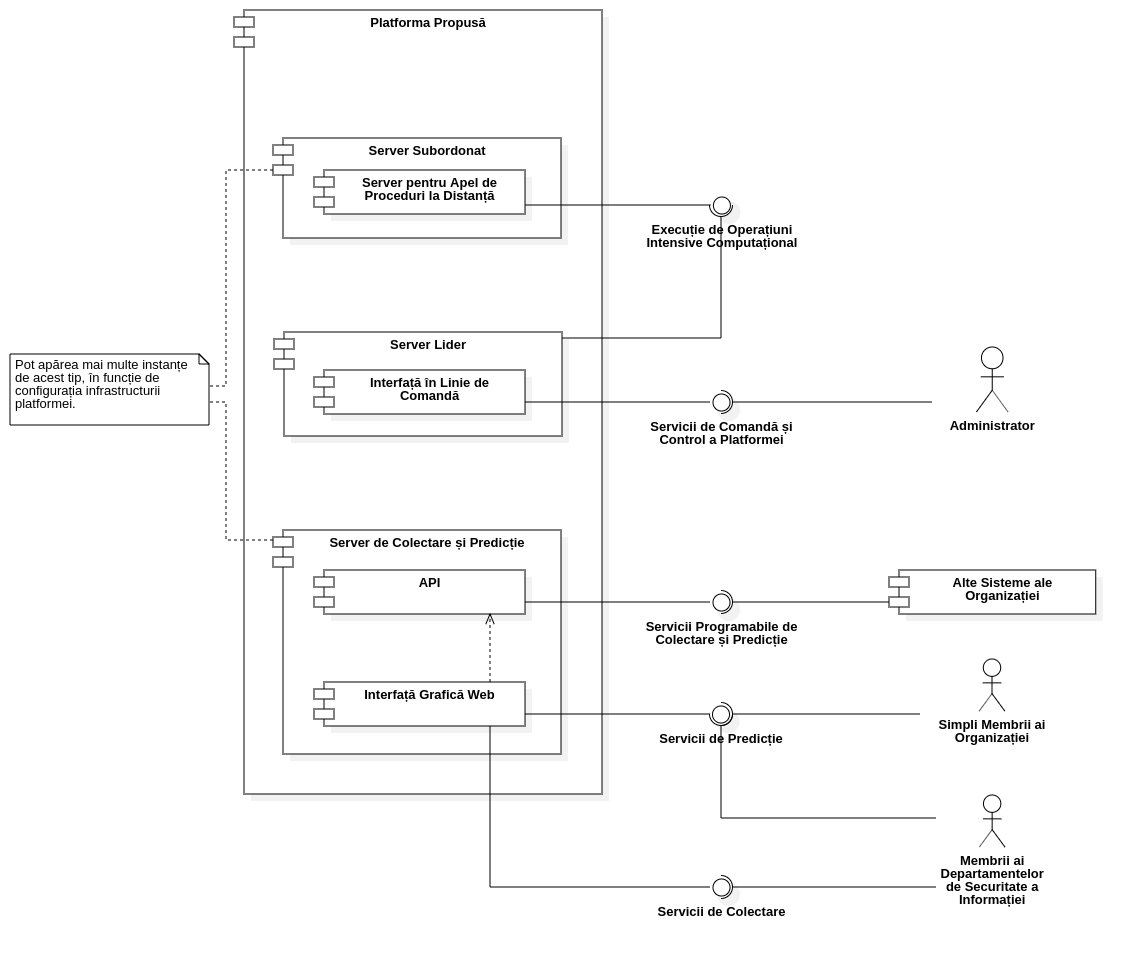
\includegraphics[width=12cm]{components/images/diagrams/component_diagram_servers.png}
    \label{fig:component_diagram_servers}
    \captionsetup{justification=centering,margin=1cm}
    \captionof{figure}{Diagramă de componente, relativă la serverele implementate}
\end{center}
\vspace{0.3cm}

\newpage

Unele dintre funcționalitățile lor sunt comune, apărând în mai multe tipuri de server în același timp. De exemplu, funcționalitatea de extragere de atribute este necesară atât serverului subordonat, care o folosește pentru procesarea fișierelor ce compun un set de date folosit pentru antrenarea unui model, cât și celui de predicție, care o utilizează pentru determinarea atributelor, pas necesar în procesul de predicție. Astfel, serverele sunt dezvoltate prin importarea în cadrul implementării lor proprii a unor componente software reutilizabile, numite \textbf{module}.

\subsection{Module}

Drumul parcurs de datele utilizatorului în interiorul platformei, de la informații brute precum fișierele benigne și malițioase și până la modelele folosite pentru a crea predicții, poate fi privit ca o \textbf{linie de asamblare}. Astfel, un \textbf{set de module} capabile să proceseze date lucrează împreună la construirea graduală a unui rezultat. Fiecare dintre ele este conectat într-o manieră secvențială la ieșirea unuia, de la care preia date de intrare, și la intrarea altuia, căruia îi predă datele sale de ieșire.

Am dedus o serie de module specifice, pe baza cerințelor funcționale mențio\-nate anterior și a modurilor în care analiza de fișiere malițioase și antrenarea de modele de învățare automată funcționează. Modulele, cât și prezența lor în fiecare tip de server, sunt listate în tabelul de mai jos.

\begin{landscape}
    \vspace*{\fill}
    \begin{table}[h]
    \centering
    \resizebox{19.5cm}{!}{
        \begin{tabular}{ | p{0.55\linewidth} | p{0.15\linewidth} | p{0.1\linewidth} | p{0.25\linewidth} | }
            \hline
            Nume & Server subordonat & Server lider & Server de colectare și predicție \\
            \hline
            Modul pentru etichetarea fișierelor și gestionarea seturilor de date & Da & Nu & Da \\
            Modul pentru extragerea atributelor din fișiere & Da & Nu & Da \\
            Modul pentru preprocesarea atributelor & Da & Nu & Da \\
            Modul pentru gestionarea modelelor de inteligență artificială & Da & Nu & Da \\
            Modul pentru gestionarea serverelor subordonate & Nu & Da & Nu \\
            \hline
        \end{tabular}
    }
    \caption{Prezența modulelor în fiecare tip de server}
    \label{tab:modules_per_servers}
\end{table}
    \vspace*{\fill}
\end{landscape}

\subsubsection{Modul pentru Etichetarea Fișierelor și Gestionarea Seturilor de Date}

Structura informațională de tip linie de asamblare are ca punct de plecare fișierele benigne și malițioase. Ele sunt identificate pe baza unei perechi de nume - tip (benign și malign) și compun setul de date principal, din care sunt selectate exemplare pentru crearea unor seturi de date folosite separat, pentru antrenarea unor modele. Fișierele provin din \textbf{alte surse de date}:

\vspace{0.3cm}

\textit{A. Set de date special creat pentru această platformă}\footnote{\href{https://github.com/iosifache/DikeDataset}{https://github.com/iosifache/DikeDataset}}

Setul de date special creat este compus, la rândul lui, din fișiere din surse publice:

\begin{itemize}
    \item \textbfit{Setul de date "Malware Detection PE-Based Analysis Using De\-ep Learning Algorithm Dataset"}\footnote{\fullcite{malware_dataset}}: Conține fișiere executabile PE benigne și malițioase.
    \item \textbfit{Proiectul MalwareBazaar}\footnote{\href{https://bazaar.abuse.ch}{https://bazaar.abuse.ch}}: Are scopul de partajare de programe mali\-țioase cu comunitatea de securitate a informației. Din cadrul acestei surse am extras fișiere OLE malițioase.
    \item \textbfit{Motorul de căutare DuckDuckGo}\footnote{\href{https://duckduckgo.com}{https://duckduckgo.com}}: L-am folosit pentru găsirea de fișiere OLE benigne, prin căutări aleatoare de documente (de exemplu, folosind șablonul \inlinecode{filetype:doc}).
\end{itemize}

Cum o procesare complet automată nu a fost posibilă, am efectuat manual o serie de pași, din linie de comandă, aceștia fiind însă replicabili prin intermediul unui script\footnote{\href{https://github.com/iosifache/DikeDataset/blob/main/others/scripts/get_files.sh}{https://github.com/iosifache/DikeDataset/blob/main/others/scripts/get\_files.sh}} realizat ulterior. Primul pas a fost cel de \textbf{descărcare}, în care toate fișierele din sursele enumerate anterior au fost salvate local, filtrate după extensie și mutate într-o structură standardizată de foldere. Fișierele au primit, în pasul de \textbf{redenumire}, un nume compus din \textit{hash}-ul lor SHA256 și o extensie aferentă tipului (\inlinecode{.exe} pentru fișierele PE și \inlinecode{.ole} pentru cele OLE).

Ținând cont de numărul de fișiere ce trebuiau scanate automat și de limitele pentru numărul maxim de scanări ce puteau fi efectuate într-un anumit interval de timp, impuse de motorul VirusTotal\footnote{\href{https://www.virustotal.com}{https://www.virustotal.com}}, am preferat utilizarea unor servicii în \textit{cloud} pentru pasul de \textbf{scanare} a fișierelor. Toate \textit{hash}-urile lor au fost salvate într-un fișier ce a fost urcat într-un spațiu de stocare din Cloud Storage, soluție software oferită de Google Cloud Platform\footnote{\href{https://cloud.google.com}{https://cloud.google.com}}. Acestea erau consumate, una câte una, de către un script implementat cu ajutorul Cloud Functions și declanșat prin intermediul unui planificator de tip Cloud Scheduler. Rezultatele, reprezentate de parți specifice ale rapoartelor de scanare cu motoare antivirus, au fost salvate într-un alt fișier. Am adăugat ulterior conținutul lui în cadrul platformei, unde rezultatele scanărilor au putut fi procesate automat pentru \textbf{etichetarea} fișierelor, proces pe care îl vom descrie mai jos.

\vspace{0.3cm}

\textit{B. Mecanism de publicare a unor rezultate de analize avansate}

În cadrul structurii de foldere folosită, apare un folder special în care fișiere (sau chiar atribute deja extrase ale unor fișiere) pot fi \textbf{publicate}, împreună cu etichetele lor. Nevoia unui astfel de mecanism apare atunci când analiștii de programe malițioase examinează în detaliu un exemplar și doresc să ajute la îmbunătățirea performanței modelelor antrenate prin oferirea unor date de încredere, care să fie folosite în cadrul unui posibil proces de reantrenare.

Publicarea poate fi realizată prin intermediul interfeței grafice și, implicit, prin intermediul API-ului. Toate datele provenite din această sursă sunt consi\-derate corecte, fișierele nemaifiind scanate cu acea componentă specifică ce apare în cazul sursei de date anterior detaliată.

Considerând componentele de care depinde învățarea automată, apare nevoia existenței unor \textbf{etichete} care ajută, prin natura și semnificația lor, modulul de inteligență artificială pentru predicția fiecăreia dintre ele:

\begin{itemize}
    \item \textbfit{Maliția}: Maliția este un indice numeric, ce indică probabilitatea ca un fișier să fie malițios. Valorile posibile sunt cuprinse între $ 0 $ și $ 1 $.
    \item \textbfit{Apartenența la familii de programe malițioase}: Acestea reprezintă, de asemenea, indici numerici pentru probabilitatea ca fișierul să aparțină de o anumită familie de programe malițioase. Valorile sunt cuprinse între $ 0 $ și $ 1 $, suma lor pentru un anumit fișier fiind egală cu $ 1 $. Familiile considerate sunt \textit{Generic}, \textit{Trojan}, \textit{Ransomware}, \textit{Worm}, \textit{Backdoor}, \textit{Spyware}, \textit{Rootkit}, \textit{Encrypter} și \textit{Downloader}.
\end{itemize}

Răspunzător pentru \textbf{etichetarea fișierelor benigne și malițioase} este primul modul al platformei. Sistemul de foldere specific acestuia permite adău\-garea manuală sau automată de fișiere noi în folderele specifice. Platforma \textbf{detectează exemplarele neavute în evidență}, prin verificarea periodică a locațiilor și a conținutului lor.

Modulul redenumește și scanează aceste fișiere, rezultatele scanărilor cu VirusTotal fiind procesate într-o manieră identică a acelora provenite de la scanarea în \textit{cloud} a întregului set de date. Cu ajutorul unei medii ponde\-rate asupra verdictului fiecărui motor antivirus, în care un vot pentru caracterul malign cântărește mai mult decât unul pentru caracterul benign, a fost determinată maliția. Etichetele atribuite de fiecare motor au fost folosite ca dovezi ale apartenenței la o anumită familie, ele fiind grupate și numărate, iar rezultatele normalizate pentru a obține probabilitățile finale.

De menționat este faptul că pentru fișierele presupuse benigne (mutate în folderul specific lor), pasul de scanare a fost sărit întrucât etichetarea este efectuată folosind valoarea $ 0 $ pentru toate etichetele considerate.

\begin{center}
    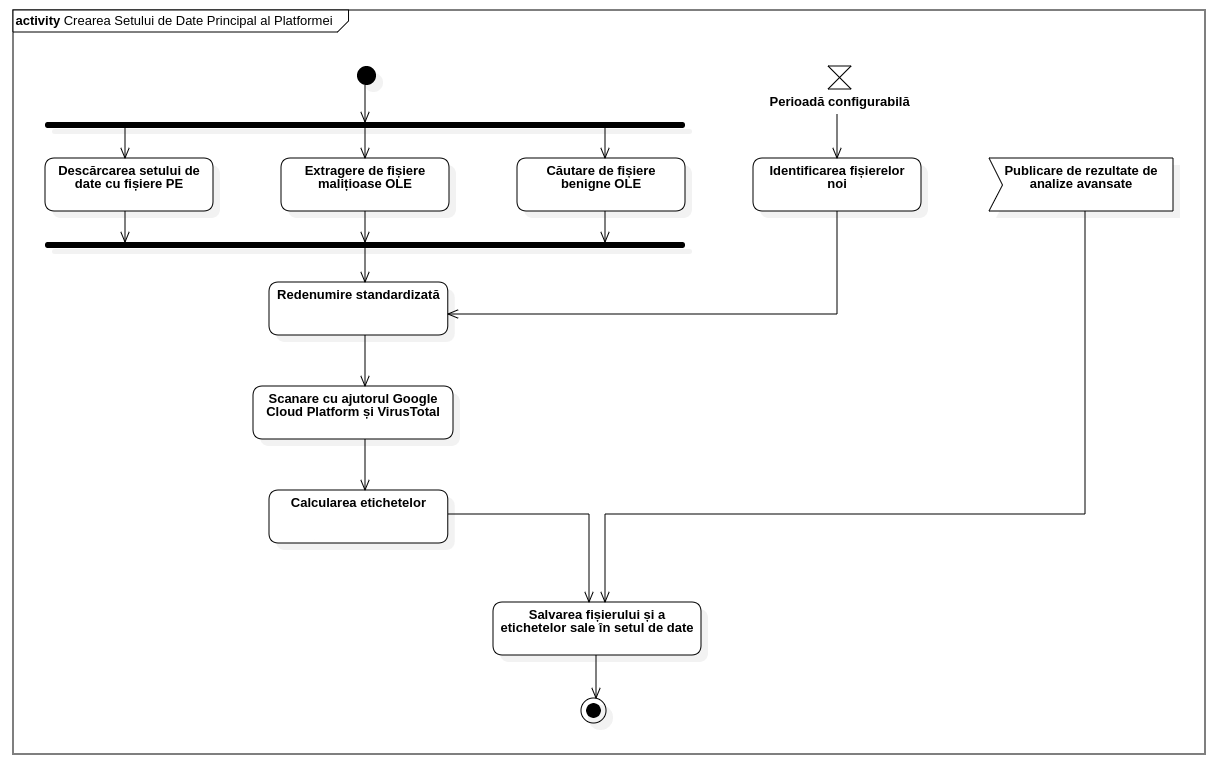
\includegraphics[width=12cm]{components/images/diagrams/activity_diagram_dataset_creation.png}
    \label{fig:activity_diagram_dataset_creation}
    \captionsetup{justification=centering,margin=1cm}
    \captionof{figure}{Diagramă de activitate pentru crearea setului de date principal}
\end{center}
\vspace{0.3cm}

Ultimul rol al acestei componente este de \textbf{a gestiona seturile de date} pe durata întregului lor ciclu de viață. Crearea unui set de date se face prin intermediul unor fișiere de configurare cu un format specific, ce cuprinde următorii parametri:

\begin{itemize}
    \item \textbfit{Formatul fișierelor}: Formatul poate fi PE sau OLE.
    \item \textbfit{Numărul de exemplare incluse}: Este un număr întreg, notat în continuare $ exemplare\_incluse $.
    \item \textbfit{Raportul dintre fișiere benigne și malițioase}: Este un număr real, cuprins între $ 0 $ și $ 1 $ și notat în continuare $ raport\_benign\_malign $.
    \item \textbfit{Maliția minimă}: Este un număr real, cuprins între $ 0 $ și $ 1 $.
    \item \textbfit{Familii de programe malițioase}: În funcție de familiile incluse în setul de date, lucru care este setat în fișierul de configurare prin specificarea lor sub forma unei liste, fiecărui fișier malițios candidat i se calculează o sumă a probabilităților de apartenență la familiile selectate. Lista se ordonează descrescător și se selectează ulterior atâtea fișiere câte au fost solicitate, și anume $ exemplare\_incluse * (1 - raport\_benign\_malign) $.
\end{itemize}

Pe baza acestor parametrii se stabilesc limite pentru caracteristicile exemplarelor și se filtrează setul de date principal al platformei. Dacă toate condițiile sunt verificate, are loc copierea detaliilor exemplarelor selectate din setul de date principal într-un set de date nou, la care apare și o linie specială, de metadate, în care sunt reținute detaliile de configurare ale acestuia.

Seturile de date pot fi citite prin operațiunea de listare a tuturor (în care se accesează numai metadatele, nu și lista de exemplare incluse) sau prin cea de citire efectivă (care apare, de exemplu, în cadrul modulului specific modelelor). În plus, sunt posibile operațiuni de actualizare, prin intermediul operației de publicare a unor rezultate, și de ștergere a seturilor de date.

\subsubsection{Modul pentru Extragerea Atributelor din Fișiere}

Primul modul inclus în procesul de antrenare a unui model de inteligență artificială este cel de extragere a atributelor. Rolul său este de a procesa fișierele benigne și malițioase, \textbf{extrăgând din cadrul lor acele caracteristici specifice}, conform cu o configurație oferită de către administrator.

La nivel arhitectural, modulul este reprezentat de o componentă care gestionează aplicarea unor sub-componente numite \textbf{extractori}. Acestea din urmă sunt capabile de a procesa numai anumite tipuri de fișiere și sunt specializate pe anumite caracteristici ale formatului de care se ocupă.

Ieșirile modulului de extragere a atributelor sunt conectate la intrările modulului următor din structura informațională de tip linie de asamblare, cel care se ocupă de preprocesarea lor. Pentru a asigura păstrarea semnificației atributelor returnate de extractorii folosiți, acestui modul i se impune o anumită configura\-ție.

Tipurile posibile de extractori sunt:

\begin{itemize}
    \item \inlinecode{StaticStrings}: Fiind un extractor de tip static, iterează prin conținutul fișierului, la nivel de octet, pentru a detecta \textbf{șirurile de caractere prin\-tabile} cu anumite lungimi și număr de apariții minime, parametrii care sunt setați în configurația platformei. Ieșirea sa constă într-o listă de șiruri de caractere printabile.
    \item \inlinecode{StaticPECharacteristics}: Neavând nevoie de rularea executabilului, acest extractor are ca ieșire \textbf{atribute specifice formatului de fișiere PE}, precum dimensiunea fișierului, funcții importate și exportate, librarii importate și detalii (nume, entropie, dimensiuni virtuale și brute) ale secțiunilor.
    \item \inlinecode{StaticOpcodes} și \inlinecode{StaticAPIs}: Extractoarele folosesc ca dezasamblor Ghidra pentru a efectua o analiză statică pentru extragerea unor liste cu toți \textbf{identificatorii codurilor de operație} găsite în cadrul executabilului analizat, respectiv cu toate \textbf{apelurile către Windows API}. Principalul dezavantaj al metodei folosite este că nu asigură aceeași credibilitate precum o analiză dinamică, în care se observă exact care sunt codurile de operație rulate sau apelurile de sistem efectuate. Astfel, în cazul unor constructe de cod repetitive sau a unor tehnici de dezasamblare (de exemplu, împachetare), extractorul nu reușește să producă o informație complet corectă.
    \item \inlinecode{DynamicOpcodes} și \inlinecode{DynamicAPIs}: Ele realizează o analiză dinamică, emu\-lând executabilele într-un mediu controlat cu ajutorul unui \textit{framework} numit Qiling\footnote{\href{https://qiling.io}{https://qiling.io}}. Au același tip de ieșire precum extractorii descriși anterior și prezintă dezavantajul că biblioteca menționată nu implementează toate apelurile de sistem disponibile în Windows\footnote{\href{https://github.com/qilingframework/qiling/issues/751\#issuecomment-822122311}{https://github.com/qilingframework/qiling/issues/751\#issuecomment-822122311}} și folosite de programele malițioase, ceea ce face ca extractorii aceștia să nu reușească să obțină rezultate utile pentru anumite fișiere executabile.
    \item \inlinecode{GeneralOLEDetails}: Acesta este un extractor care analizează static fișie\-rul Office, extrăgând \textbf{detalii generale ale formatului OLE}. Ele variază de la text găsit în anteturi, număr de pagini și cuvinte, timpi de creare și modificare, indicatori (engl. "\textit{flags}"), numărul de obiecte de tip Flash și de sectoare, cât și detalii (nume și dimensiune) ale intrărilor în directoare (engl. "\textit{directory entry}").
    \item \inlinecode{OLEMacros}: Parcurge fișierul OLE în căutarea de \textbfit{macro}-uri VBA. Ieșirea sa este reprezentată de o listă cu codul sursă pentru fiecare \textit{macro} identificat.
\end{itemize}

\vspace{0.3cm}
\begin{center}
    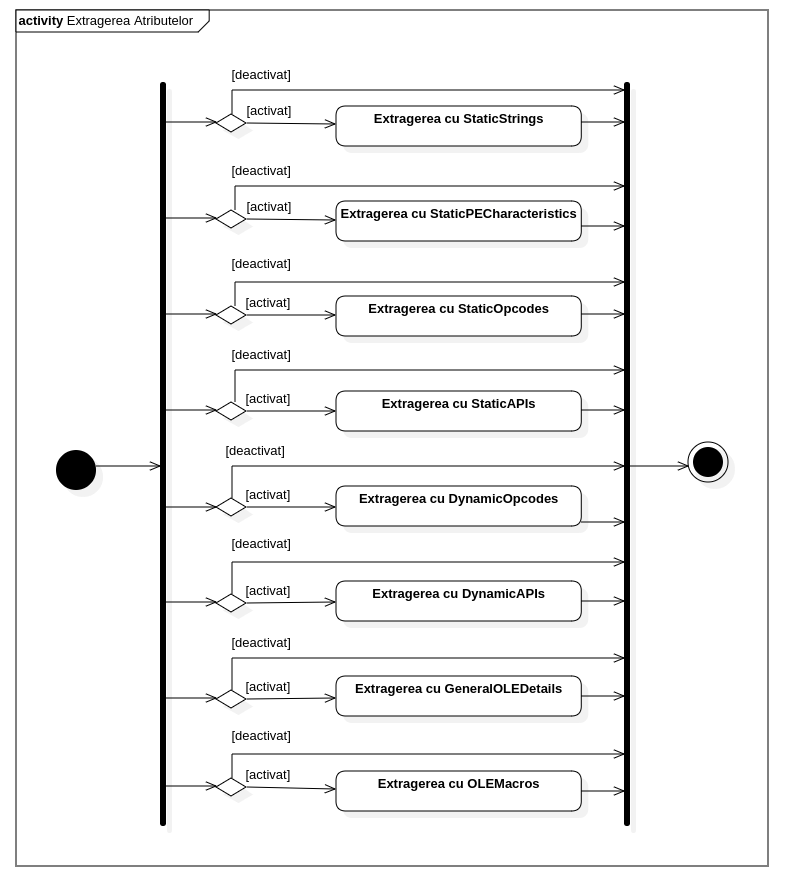
\includegraphics[width=8cm]{components/images/diagrams/activity_diagram_attribute_extraction.png}
    \label{fig:activity_diagram_attribute_extraction}
    \captionsetup{justification=centering,margin=1cm}
    \captionof{figure}{Diagramă de activitate pentru extragerea atributelor}
\end{center}

\subsubsection{Modul pentru Preprocesarea Atributelor}

După ce toate atributele brute au fost determinate cu ajutorul modulului de extragere, ele sunt preluate sub formă matriceală (în care fiecare linie reprezintă un exemplar, iar coloanele tipuri de atribute) de modulul de preprocesare pentru \textbf{a le transforma în reprezentări mai adecvate învățării automate}.

Asemenea predecesorului său, acest modul aplică sub-componente de transformare, numite \textbf{preprocesoare}, specializate pe un anumit tip de atribute și selectate în funcție de ieșirile extractorilor. Fiecare preprocesor implementează operații specifice, pe care le aplică la nivelul atributelor de care este respon\-sabil. De menționat este că premergător se asigură inexistența unor valori lipsă în setul de date, printr-un proces de \textbf{imputare} cu valori fixe, specifice tipului de date al atributului.

Preprocesoarele implementate sau importate din biblioteca \inlinecode{scikit-learn}\footnote{\href{https://sklearn.org}{https://sklearn.org}} sunt:

\begin{itemize}
    \item \inlinecode{Identity}: Replică datele de intrare la ieșire.
    \item \inlinecode{Binarizer}: Binarizează datele conform cu o limită stabilită.
    \item \inlinecode{KBinsDiscretizer}: Grupează date continue în intervale.
    \item \inlinecode{Counter}: Numără elementele componente ale unui atribut.
    \item \inlinecode{CountVectorizer}: Transformă un text într-o matrice de numere de apari\-ții pentru fiecare cuvânt.
    \item \inlinecode{NGrams}: Numără grupuri de caractere consecutive, care apar într-o fe\-reastră de o lungime oferită ca parametru. Cum pentru lungimi mai mari numărul de atribute devine mare, toate literele textului pot fi opțional transformate în minuscule și selectat un set de caractere mai restrâns.
    \item \inlinecode{GroupCounter}: Calculează, pentru fiecare grup, numărul de elemente incluse în el. Grupurile și elementele copii sunt precizate în configurația preprocesorului. În cadrul platformei, au fost definite grupuri pentru coduri de operații executate de procesor (de exemplu, \inlinecode{call} și \inlinecode{ret} sunt conside\-rate operațiuni de lucru cu stiva) și pentru funcții exportate de Windows API (de exemplu, grupul de funcții criptografice include apeluri precum \inlinecode{CertOpenStore} și \inlinecode{CryptCreateHash}), ultimele fiind preluate din cadrul unei implementări\footnote{\href{https://github.com/Hullgj/report-parser}{https://github.com/Hullgj/report-parser}} cu sursă deschisă a unui articol științific\footnote{\fullcite{randep}}.
    \item \inlinecode{SameLengthImputer}: Aduce toate atributele exemplarelor la aceeași lungi\-me, fie la una stabilită ca parametru, fie a exemplarului cu cea mai mare lungime.
\end{itemize}

După ce toate preprocesoarele sunt aplicate, toate informațiile rezultate sunt de tip numeric. Ele sunt \textbf{scalate} în intervalul $ [0, 1] $, unde pe valoarea $ 0 $ este proiectată valoarea minimă găsită în interval și pe $ 1 $ valoarea maximă. Acest procedeu asigură "\textit{o viteză mai mare de învățare}" și că "\textit{intrările se află într-un interval relativ mic, pentru a evita problemele pe care le au calculatoarele când lucrează cu numere foarte mari sau foarte mici}" \cite{hundred_page_ml}.

Ultima operațiune efectuată în cadrul acestui modul, înainte ca datele să fie oferite următorului cu scopul de a se efectua o antrenare a unui model pe baza lor, este \textbf{reducerea dimensionalității}. Motivul este că algoritmii lucrează mai eficient (mai rapid și cu o acuratețe mai mare) atunci când procesează o "\textit{informație de dimensionalitate redusă, care rezumă informația din spațiul inițial al atributelor}"\footnote{\fullcite{ml_feature_engineering}}.

Un exemplu relevant numărului mare de atribute la care se poate ajunge este cazul aplicării peste rezultatul unui extractor \inlinecode{StaticStrings} a unui preprocesor \inlinecode{NGrams}, având setate parametrul $ N = 2 $ și alfabetul englez de minuscule (cu lungime de $ 26 $ de caractere). Astfel, lungimea vectorului de atribute returnat este de $ 26^2 = 676 $, dintre care multe valori sunt redundante (care sunt $ 0 $ pentru toate exemplarele analizate sau care au o variație infimă).

Pentru toți algoritmii de reducere a dimensionalității, numărul de atribute returnate este determinat în funcție de un parametru configurabil care indică variația minimă ce trebuie înglobată în toate acestea sau numărul total de atribute create. Algoritmii selectați sunt:

\begin{itemize}
    \item \textbfit{Analiza Componentelor Principale} (engl. "\textit{principal component ana\-lysis}" și abreviat PCA): Presupune determinarea unei baze în care toți vectorii unitate sunt ortogonali și care reprezintă cel mai bine variația datelor. După, se transformă datele în această nouă bază și se selectează cele mai relevante atribute.
    \item \textbfit{Factorizarea în Matrice Non-negative} (engl. "\textit{non-negative matrix factorization}" și abreviat NMF): Găsește două matrice non-negative, de dimensiuni $ m * o $ și $ o * n $, a căror produs să aproximeze matricea non-negativa a atributelor, de dimensiuni $ m * n $. Atributele relevante sunt chiar cele reprezentate de dimensiunea $ o $ a celor doua matrice găsite.
    \item \textbfit{Analiza Componentelor Independente} (engl. "\textit{independent component analysis}" și abreviat ICA): Găsește componentele independente din care fiecare atribut este presupun ca fiind compus.
\end{itemize}

\begin{center}
    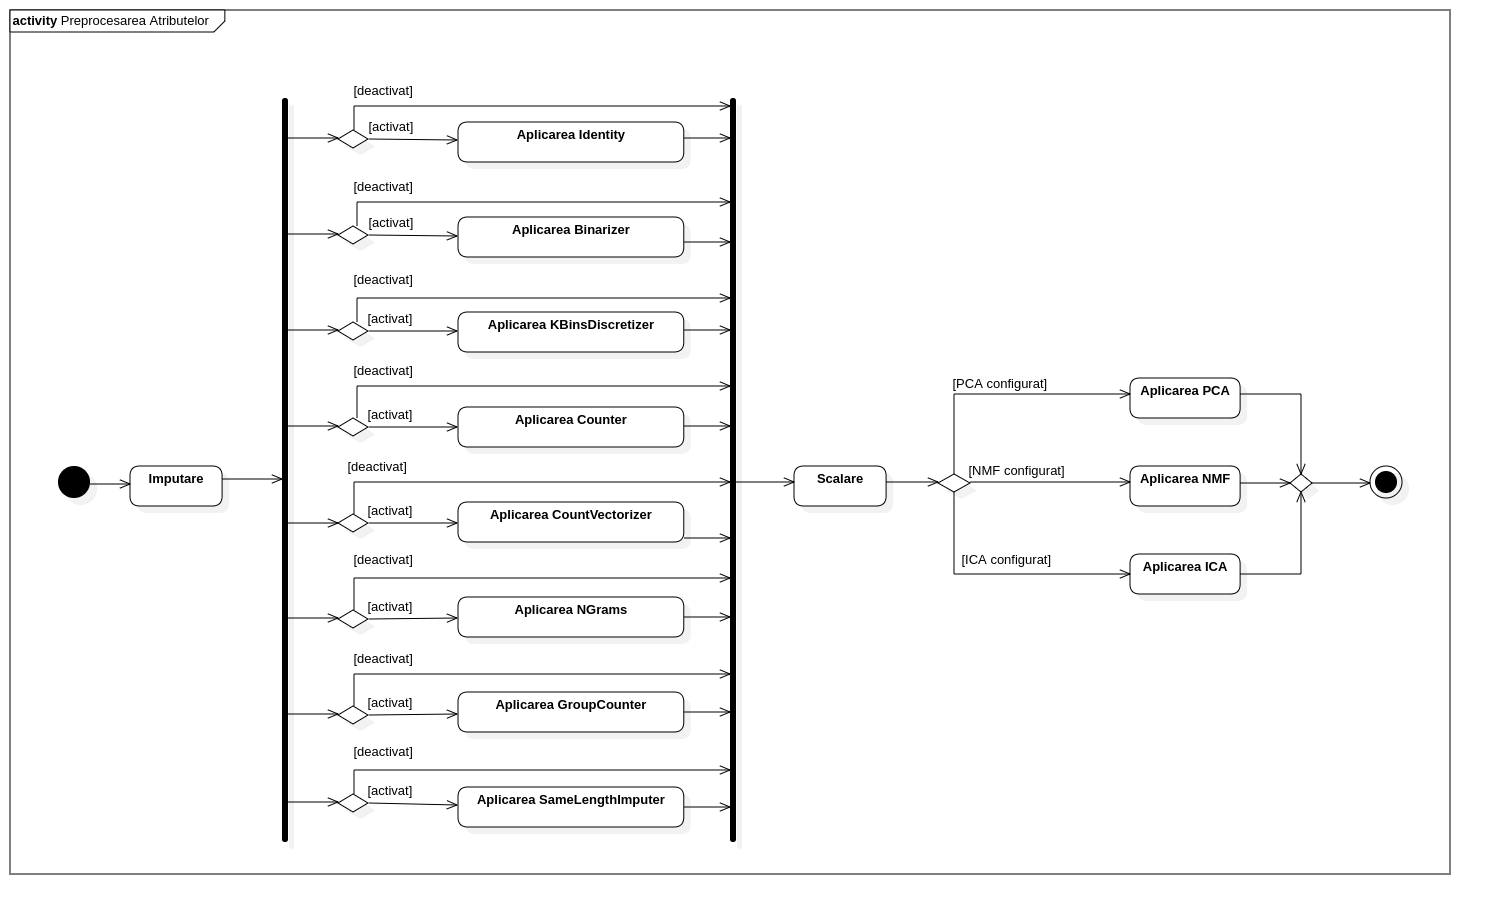
\includegraphics[width=12cm]{components/images/diagrams/activity_diagram_attribute_preprocessing.png}
    \label{fig:activity_diagram_attribute_preprocessing}
    \captionsetup{justification=centering,margin=1cm}
    \captionof{figure}{Diagramă de activitate pentru preprocesarea atributelor}
\end{center}
\vspace{0.3cm}

\subsubsection{Modul pentru Gestionarea Modelelor de Inteligență Artificială}

Atributele procesate sunt folosite în continuare ca date de intrare pentru \textbf{antre\-narea unui model de inteligență artificială}.

Crearea unuia pleacă de la un fișier de configurare cu format special, în care sunt specificate și detaliile configurării modulelor de extragere și de preprocesare a atributelor astfel:

\begin{itemize}
    \item \textbfit{Setul de date}: Indică ce set de date este folosit pentru antrenarea mode\-lului.
    \item \textbfit{Obiectivul modelului}: Tipurile au fost stabilite prin preluarea celor mai întâlnite obiective din publicațiile de actualitate \cite{ml_malware_survey}. Ele indică de ce natură sunt datele de ieșire ale modelului. Primul obiectiv este cel de \textbf{regresie a maliției}, prin care, pe baza atributelor fișierului, i se prezice maliția. Următorul este cel de \textbf{clasificare}, prin care un fișier este încadrat probabilistic în mai multe familii de programe malițioase. Ultimul obiectiv, inclus automat în cele anterioare, este reprezentat de \textbf{analiza de similaritate}, prin care atributele exemplarului nou, trimis spre a fi ana\-lizat, sunt comparate cu atributele celor aflate în setul de date și sunt astfel selectate exemplarele care obțin cel mai mare scor de similaritate Pearson.
    \item \textbfit{Listă de extractori}: Pentru fiecare, apare și o listă de preprocesoare atașați.
    \item \textbfit{Algoritmul de reducere a dimensionalității}: Este numele de identificare al algoritmului folosit.
    \item \textbfit{Configurația algoritmului de reducere a dimensionalității}: Poate fi numărul caracteristicilor selectate de algoritmul de reducere a dimensionalității sau variația minimă înglobată de acestea (numai pentru PCA).
    \item \textbfit{Raportul dintre numărul de exemplare folosite pentru antrenare și a acelora din tot setul de date}: Acest număr întreg, între $ 0 $ și $ 1 $, este folosit la împărțirea setului de date folosit.
    \item \textbfit{Algoritmul de învățare automată}: Este numele de identificare al algoritmului folosit.
\end{itemize}

Algoritmii de învățare automată folosiți sunt unii de regresie. Aceștia se pretează atât pe regresia maliției, cât și pe clasificarea exemplarelor pe familii întrucât aceasta este cu etichete multiple și limite moi (engl. "\textit{soft multi-label}"). Acest caracter presupune că se va returna, pentru fiecare clasă pentru care există etichete, o probabilitate de apartenență a fișierului analizat în ea, condiția fiind aici ca suma lor să fie $ 1 $. Algoritmii selectați aparțin de categoria supervizată și sunt:

\begin{itemize}
    \item \textbfit{Regresie pe bază de arbori de decizie}: Estimează un rezultat prin verificări repetate ale unor condiții până când modelul este suficient de încrezător pentru a face o predicție.
    \item \textbfit{Mașini cu vectori de suport} (engl. "\textit{support vector machines}"): Folosește conceptul de vectori de suport pentru determinarea unui hiperplan ce minimizează erorile.
    \item \textbfit{Păduri aleatoare} (engl. "\textit{random forests}"): Antrenează o multitudine de arbori de decizie și folosește pe post de predicție media predicțiilor individuale ale fiecărui arbore, cu scopul de a îmbunătăți acuratețea și de a controla supraînvățarea.
\end{itemize}

După ce fișierul este citit, are loc \textbf{divizarea în două a setului de date}, format din atributele procesate. Primul, cel de antrenare, este folosit numai pentru antrenarea modelului, în timp ce al doilea, cel de test, este folosit pentru evaluarea rezultatelor modelului selectat.

Antrenarea modelului se efectuează conform procedeului de \textbf{validare în\-crucișată}, pe setul de date specific, prin antrenări succesive de modele. Selectarea modelului final se face prin alegerea celui care obține cea mai mică eroare medie pătratică.

\vspace{0.3cm}
\begin{center}
    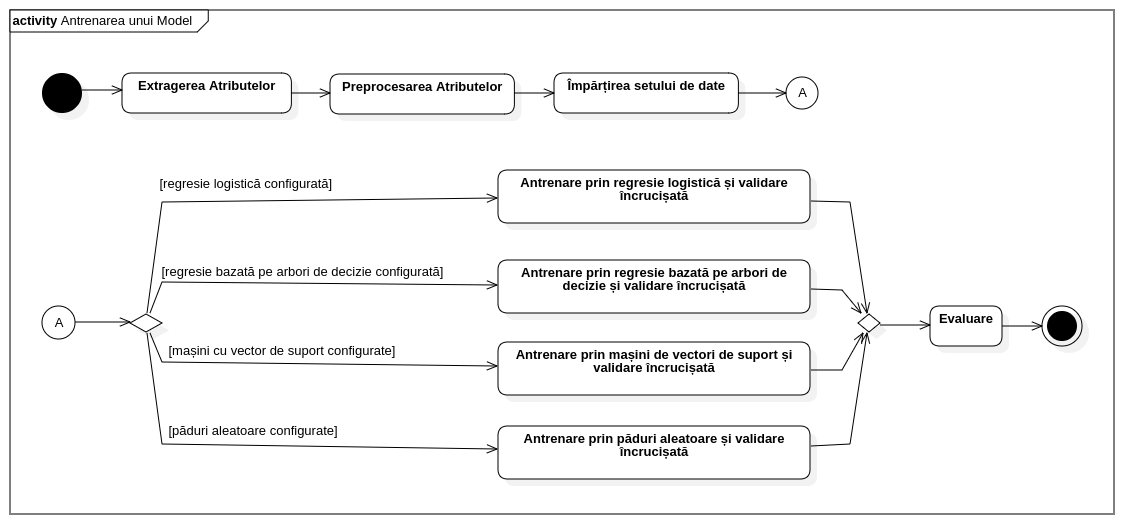
\includegraphics[width=12cm]{components/images/diagrams/activity_diagram_model_training.png}
    \label{fig:activity_diagram_model_training}
    \captionsetup{justification=centering,margin=1cm}
    \captionof{figure}{Diagramă de activitate pentru antrenarea unui model}
\end{center}

Antrenarea unui model declanșează o \textbf{evaluare avansată} a acestuia, pe baza unor seturi de criterii specifice obiectivului său. Pentru modelele de regresie a maliției, se determină eroarea maximă, eroarea medie, eroarea medie pătratică și scorul $ R^2 $. Pe lângă acestea, pentru toate predicțiile efectuate, se determină eroarea absolută și se grupează în cadrul unei histograme.

Din cauza caracterului modelele de clasificare utilizate în cadrul platformei, pentru fiecare etichetă specifică unei familii de programe malițioase, este oferită o valoare probabilistică într-un spațiu continuu. Astfel, este necesară o relativizare în ceea ce privește rezultatele prezise, pentru a putea aplica metodele clasice de evaluare la nivel de clasă (prin alegerea unei clase anume) și la nivel de valoare (prin stabilirea unei limite pentru binarizarea etichetelor returnate, peste care un exemplar este considerat ca aparținând de familia în cauză). Datorită caracterului continuu al valorilor prezise, sunt generate în primul rând, pentru fiecare clasă, metricile specifice regresie. Ulterior, clasele sunt binarizate conform cu limita stabilită pentru a calcula metrici specifice clasificărilor: matrice de confuzie, acuratețe, predicție, reamintire și coeficientul de corelație al lui Matthews.

Modelele antrenate și evaluate pot fi folosite ulterior în producție, pentru \textbf{prezicerea unor rezultate} pentru fișiere ce nu au mai fost procesate până în acel moment de model. Cum timpul de extragere a atributelor poate fi unul ridicat din cauza tipului de analiză efectuat, predicția a fost divizată în doua etape. Prima este de creare a unui tichet prin specificarea fișierului analizat, a modelului și a configurației folosite. Urmează o etapă de verificare, care poate returna fie un rezultat nul, dacă predicția pentru fișierul în cauză nu este finalizată, fie rezultatul predicției în cazul contrar.

Acuratețea modelelor poate fi crescută folosind mecanismul de publicare de rezultate ale unor analize detaliate în combinație cu cel de \textbf{reantrenare} a modelelor. Acesta din urmă poate fi atât instant, la comanda administratorului, cât și periodic, prin stabilirea unui interval la care reantrenarea să aibă loc.

Alte operațiuni disponibile sunt cele specifice gestionării de modele: listare, actualizarea unor parametrii folosiți în clasificarea (în fișier curat, suspect sau malițios) unui fișier în funcție de maliția prezisă pentru el și ștergere.

\subsubsection{Modul pentru Gestionarea Serverelor Subordonate}

După cum am descris anterior, platforma are o arhitectura cu lider și subordo\-nați, în care un server central deleagă operațiuni intensive computațional unor servere capabile din punct de vedere al resurselor. Toate problemele care intervin în procesul de gestionare a acestora sunt rezolvate în cadrul unui modul, folosit numai de către serverul lider.

În primul rand, el se ocupa de \textbf{gestionarea conexiunilor} dintre serverul lider și cele subordonate. Cum ultimele au servicii RPC, ce ascultă pe un port anume, modulul oferă posibilitatea administratorului de a se conecta la un server anume, condiția fiind ca el să cunoască perechea de adresă - port. Alte opțiuni sunt de a scana o rețea întreagă (cu scopul de a se conecta la toate serverele identificate) și de listare a conexiunilor active.

Pe de alta parte, modulul joacă \textbf{rol de dispecer}, folosind o listă de conexiuni și un algoritm de planificare de tip Round Robin. Atunci când o sarcină trebuie delegată, el verifică următorul server din listă, după cel căruia i-a fost atribuită o sarcină la ultima execuție. În cazul în care acesta este liber (nu execută în acel moment o altă sarcină), sarcina îi este atribuită lui. Altfel, cursorul din listă este avansat până la găsirea unui server liber sau la finalizarea interogării tuturor serverelor. În ultimul caz, în care toate sunt ocupate, planificarea se încheie fără succes, iar sarcina este abandonată.

Abordarea descrisă anterior are avantajul de a evita apariția unor serverele care nu vor executa niciodată o sarcină. De exemplu, dacă lista era parcursă de la început spre final, liniar și fără ciclicitate, iar sarcinile erau suficient decalate între ele pentru a le asigura execuția completă, primele servere din listă erau solicitate constant, în timp ce ultimele rămâneau inactive pentru totdeauna.

\begin{center}
    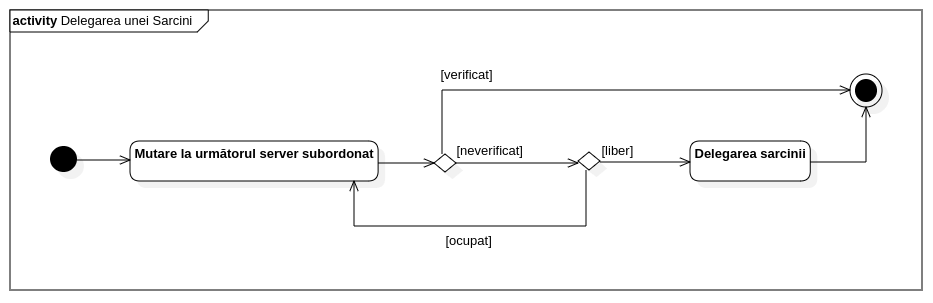
\includegraphics[width=12cm]{components/images/diagrams/activity_diagram_task_delegation.png}
    \label{fig:activity_diagram_task_delegation}
    \captionsetup{justification=centering,margin=1cm}
    \captionof{figure}{Diagrama de activitate pentru delegarea unei sarcini}
\end{center}
\vspace{0.3cm}

\newpage

De menționat este că \textbf{sarcinile} pot fi de două tipuri: sincrone, în care serverul lider așteaptă finalizarea execuției cu scopul de a-i procesa rezultatul (de exemplu, afișare pe ecran), și asincrone, în care serverul lider continuă să preia comenzi de la administrator și serverul delegat să își execute sarcina.

\section{Testare}
\label{sec:platform_testing}

Am efectuat o \textbf{testare semi-automată a platformei}, asemănătoare conceptual cu cea de \textbf{integrare ascendentă}. Dezvoltarea a plecat de la modulele individuale, care nu depindeau de altele, și a continuat cu cele ce aveau legături cu modulele deja implementate. Pentru fiecare etapă a dezvoltării, am realizat \textit{script}-uri pentru testarea funcționalității modulului implementat și, implicit, a eventualelor legături cu alte. Rezultatele acestora au fost verificate manual, asigurând corectitudinea lor.

După implementarea modulelor și a componentelor platformei care pot comunica direct cu utilizatorii, le-am asigurat o testare manuală prin:

\begin{itemize}
    \item Rularea în linie de comandă a comenzilor interfeței administratorului;
    \item Apelarea din linie de comandă, cu ajutorul clientului HTTPie\footnote{\href{https://httpie.io}{https://httpie.io}}, a rutelor API-ului; și
    \item Verificarea în \textit{browser} a funcționalităților disponibile în interfața grafică web.
\end{itemize}

Am ținut cont de posibilele înlănțuiri ce pot apărea între comenzi, apeluri de rute ale API-ului sau funcționalități din interfața grafică web întrucât acestea sunt capabile, de regulă, de a duce un program într-o stare impredictibilă, în care funcționarea nu mai este corectă. În plus, la fiecare modificare a codului sursă în urma descoperirii unei funcționări necorespunzătoare, am efectuat \textbf{testare de regresie}, asigurându-ne că platforma are un comportament complet determinist.

Menționăm faptul că API-ul a fost testat și cu ocazia integrării soluției software în cadrul unui alt program, numit \textbf{DACIA}. Acesta a fost dezvoltat în limbajul de programare C++, pentru proiectul de cercetare "\textit{Sistem de detecție a atacurilor cibernetice asupra sistemelor informatice folosind tehnici de inteligen\-ță artificială}", realizat în Academia Tehnică Militară "\textit{Ferdinand I}" București. Funcționalitatea programului este de a scanare orice fișier dintr-un folder moni\-torizat, cu ajutorul unei serii de motoare antivirus printre care se numără și platforma prezentată în această lucrare.

\end{document}